\section{Scene Backgrounds}
\label{app:scenes}

The difficulty of detecting a marker in a scene differs depending on the background.
If the background contains similar features to the marker, the marker will detect more similar points it has to sort out.
This kind of noise is hard to simulate.
To test how the detector performs, all the different backgrounds are used.
In figure \ref{fig:backgrounds} is the backgrounds shown.

\begin{figure}[h]
\centering
  \begin{subfigure}{\exampleWidth}  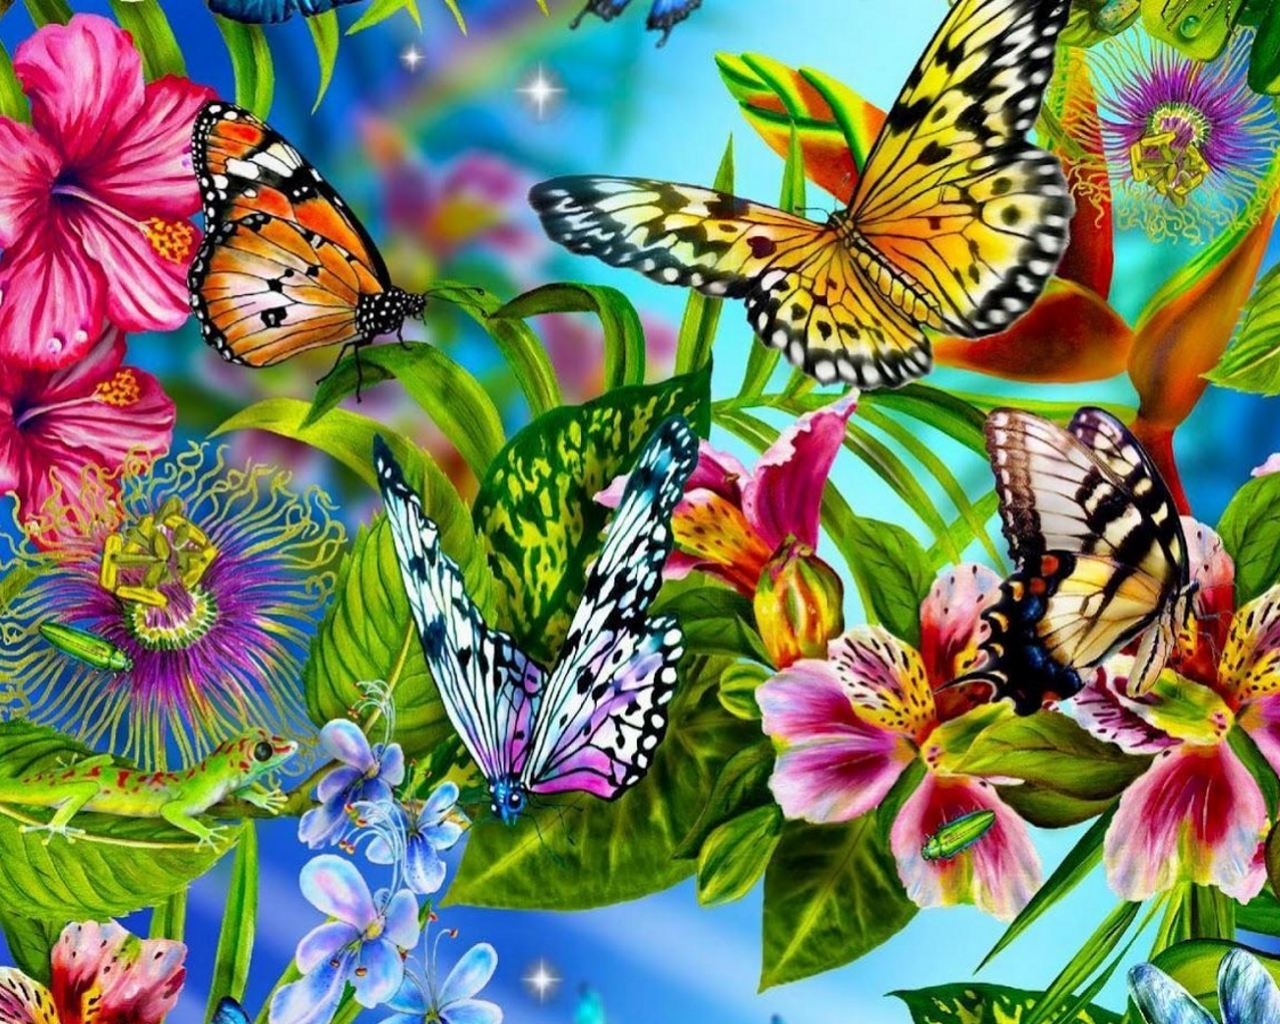
\includegraphics[width=\linewidth]{graphics/color1}   \caption{Many butterflies.} \label{fig:scene_m_but}  \end{subfigure}
  \begin{subfigure}{\exampleWidth}  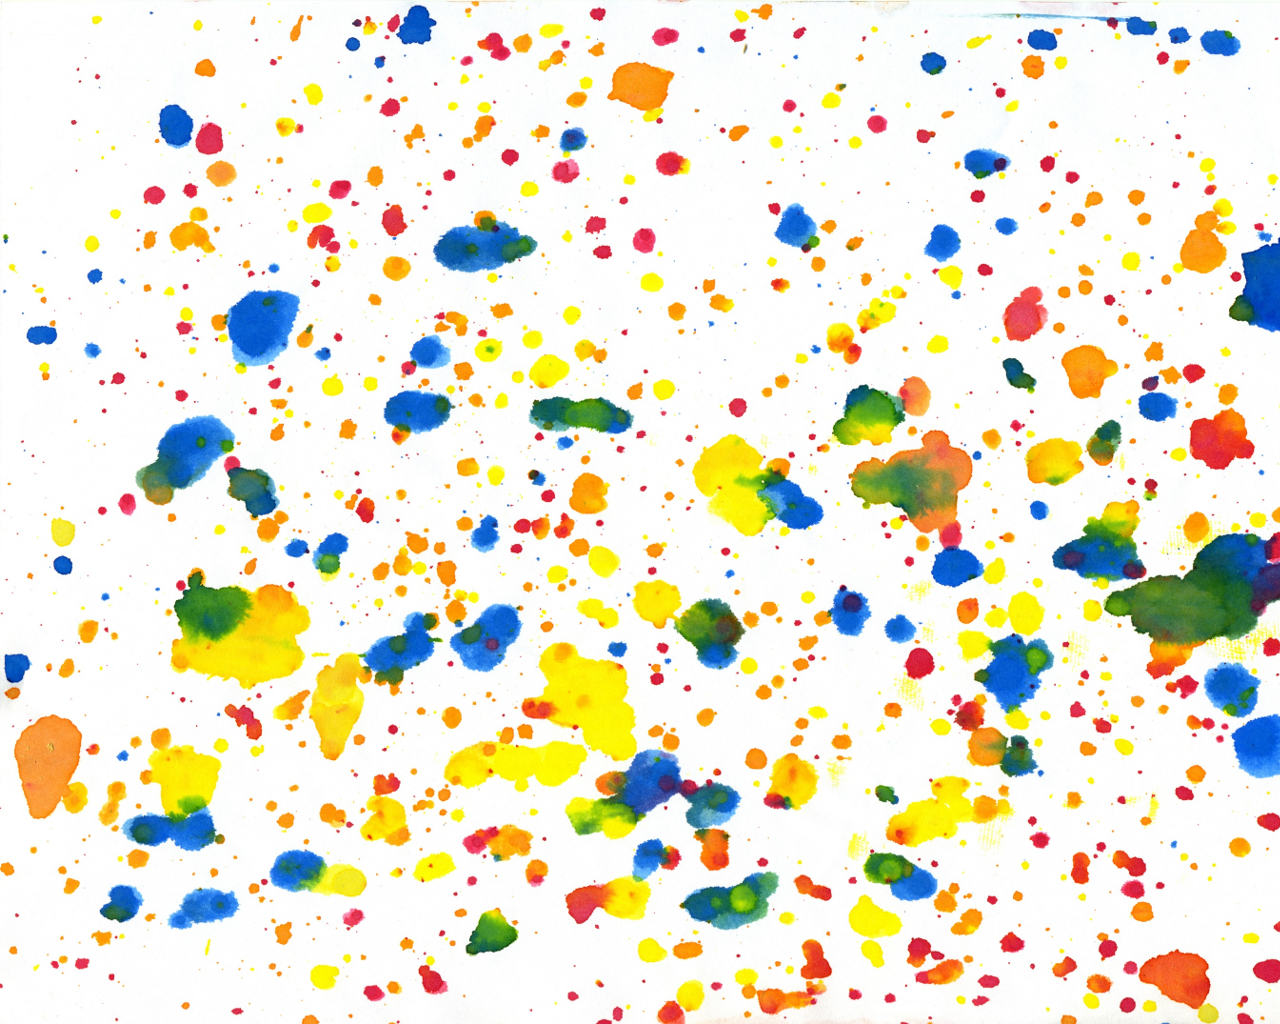
\includegraphics[width=\linewidth]{graphics/color2}   \caption{Color spots.}      \label{fig:scene_spots}  \end{subfigure}
  \begin{subfigure}{\exampleWidth}  
\includegraphics[width=\linewidth]{graphics/color3}   \caption{One butterfly.}    \label{fig:scene_s_but}  \end{subfigure}
  \begin{subfigure}{\exampleWidth}  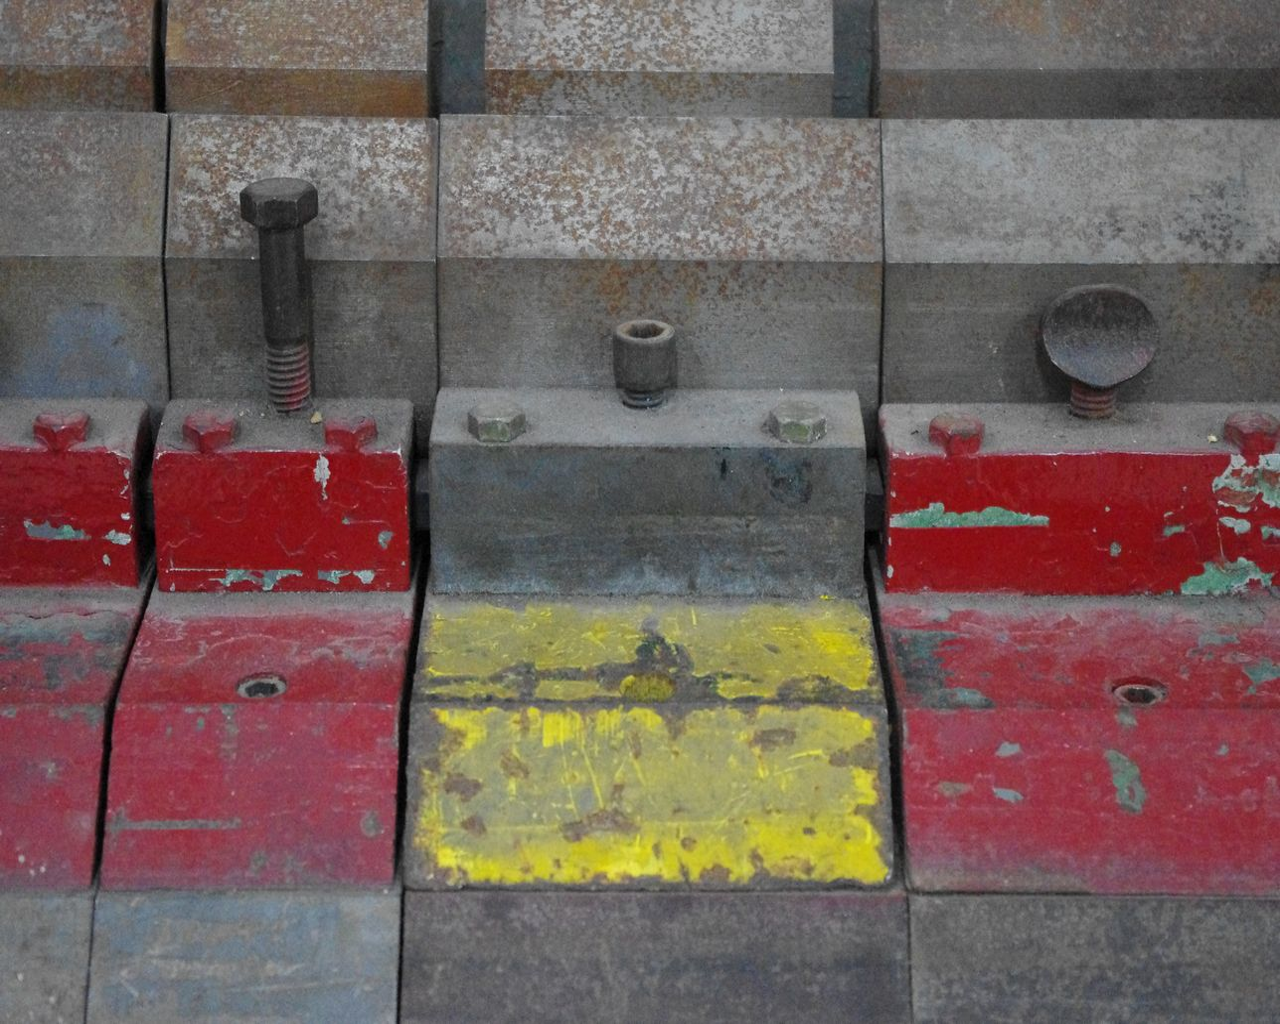
\includegraphics[width=\linewidth]{graphics/lines1}   \caption{Metal.}            \label{fig:scene_metal}  \end{subfigure}
  \begin{subfigure}{\exampleWidth}  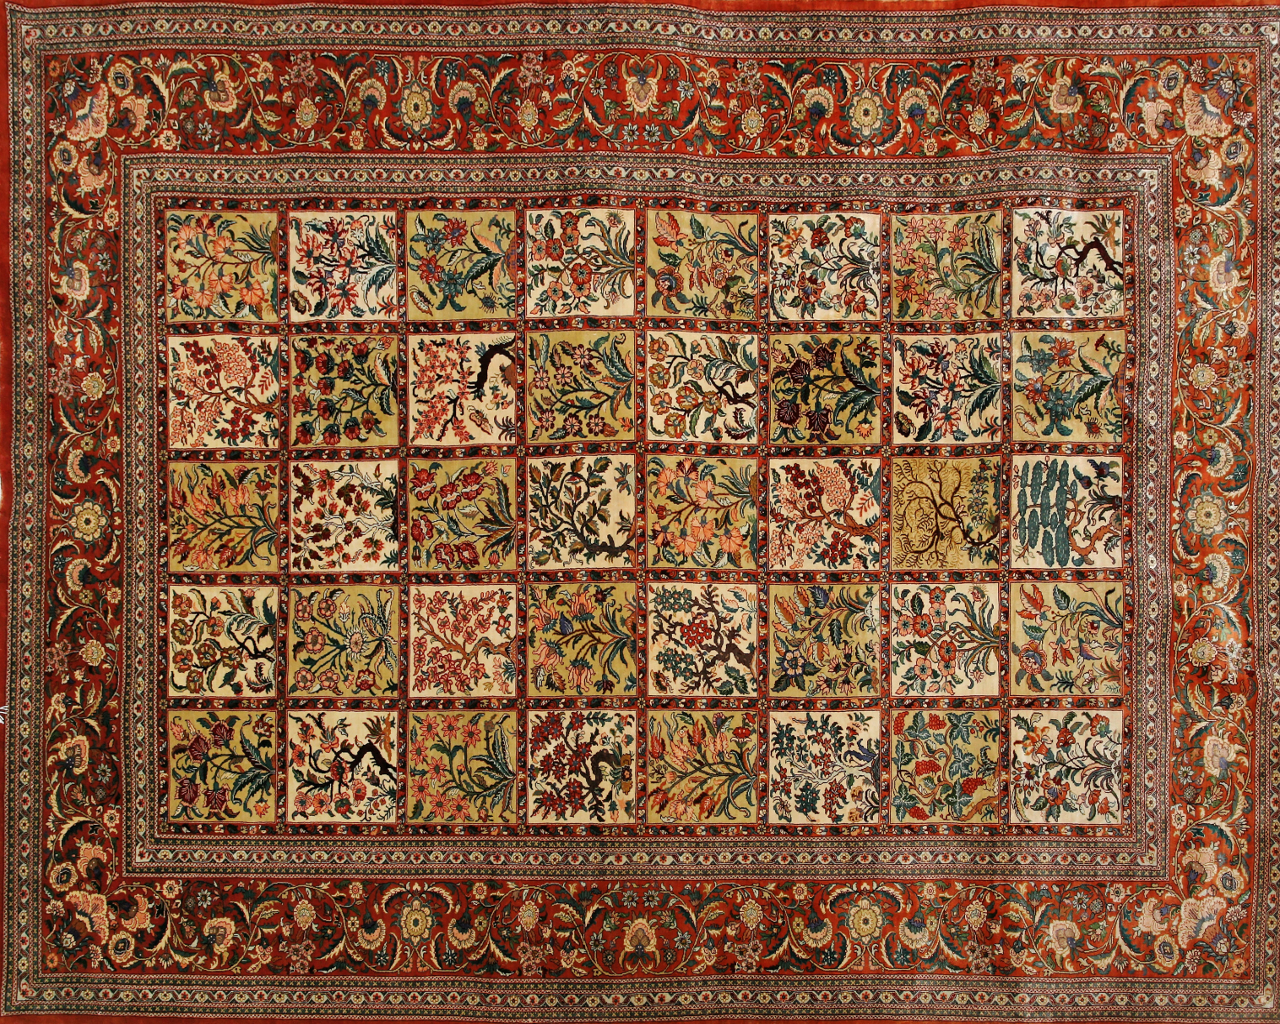
\includegraphics[width=\linewidth]{graphics/texture1} \caption{Carpet.}           \label{fig:scene_carpet} \end{subfigure}
  \begin{subfigure}{\exampleWidth}  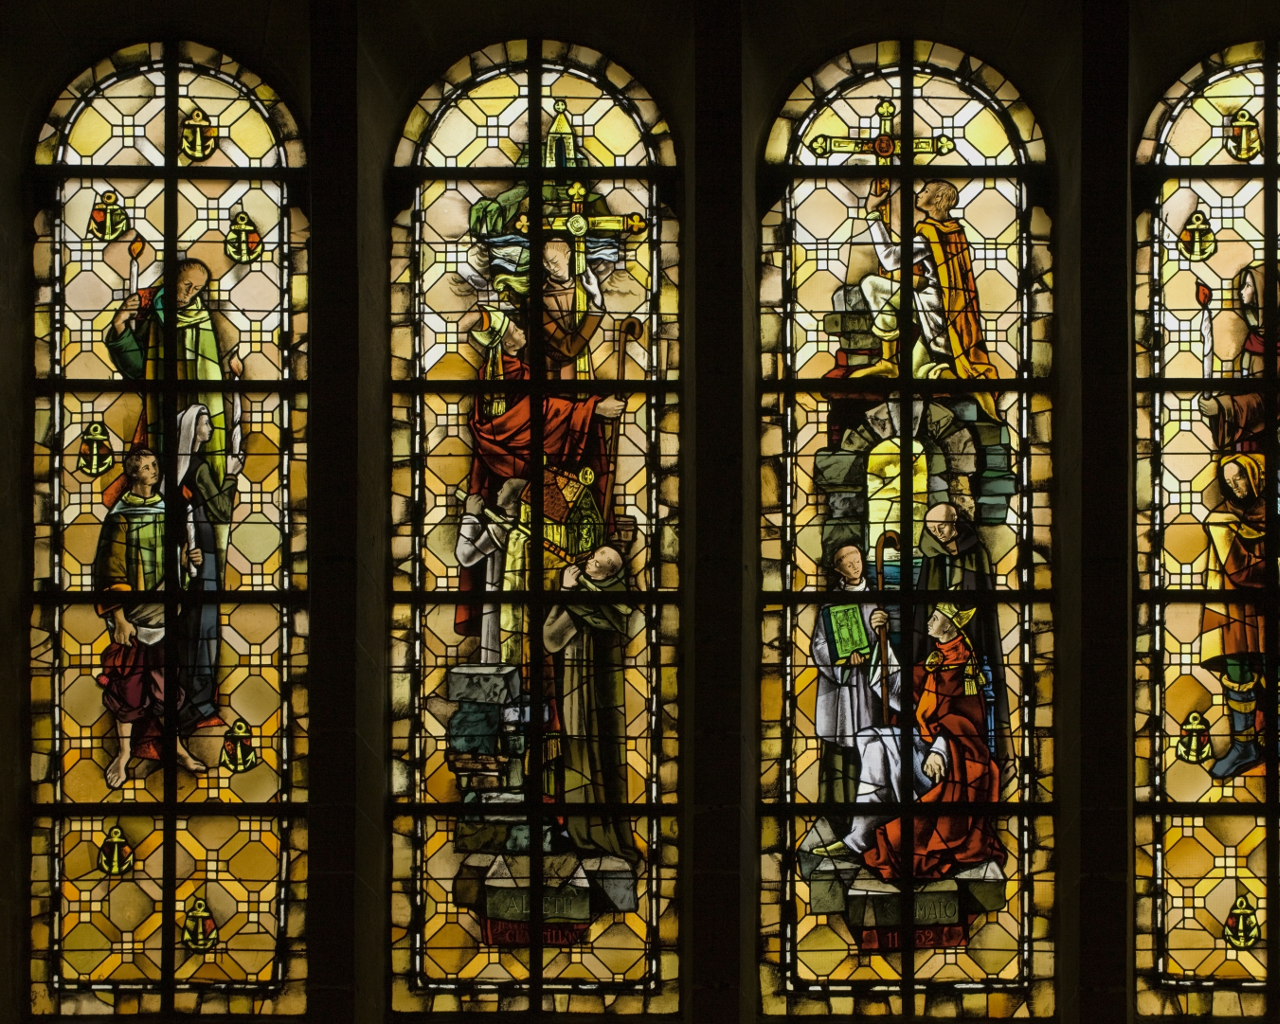
\includegraphics[width=\linewidth]{graphics/texture2} \caption{Mosaik window.}    \label{fig:scene_mosaik} \end{subfigure}
  \begin{subfigure}{\exampleWidth}  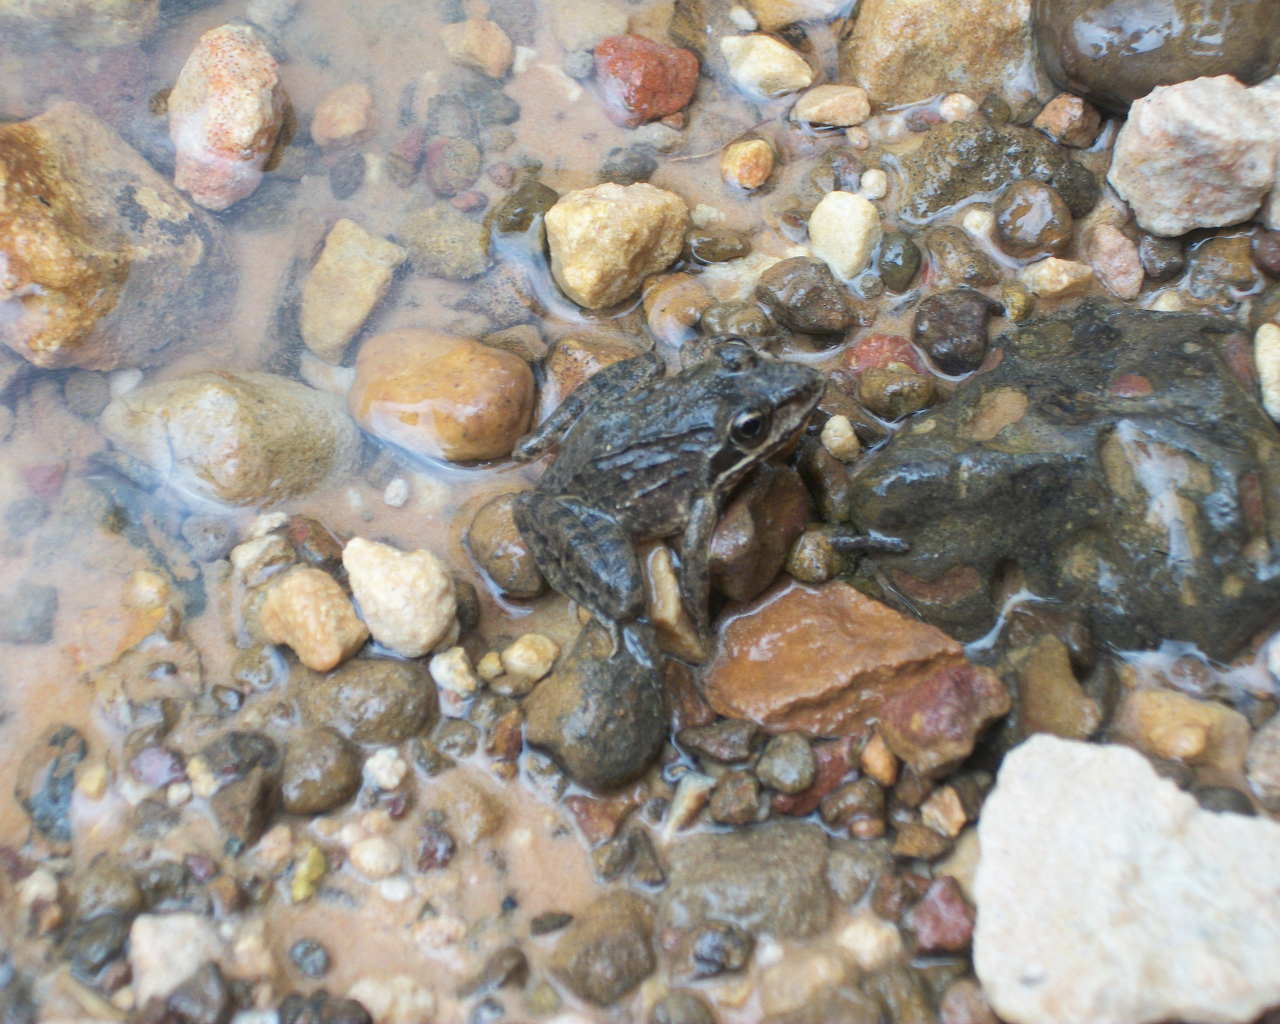
\includegraphics[width=\linewidth]{graphics/texture3} \caption{Waterbed.}         \label{fig:scene_waterb} \end{subfigure}
  \caption{The images used as a test for background noise when detecting images.}
  \label{fig:backgrounds}
\end{figure}

\section{Robotics Plots}
\label{app:roboticsPlots}

Robot configurations of the robot when tracking one or three points at the three different speeds.
The slow speed can be seen in figure \ref{fig:robotic_conf_slow_1pt} and \ref{fig:robotic_conf_slow_3pt}, 
the medium speed can be seen in figure \ref{fig:robotic_conf_medium_1pt} and \ref{fig:robotic_conf_medium_3pt},
the fast speed can be seen in figure \ref{fig:robotic_conf_fast_1pt} and \ref{fig:robotic_conf_fast_3pt}.

\begin{figure}[H]
\centering
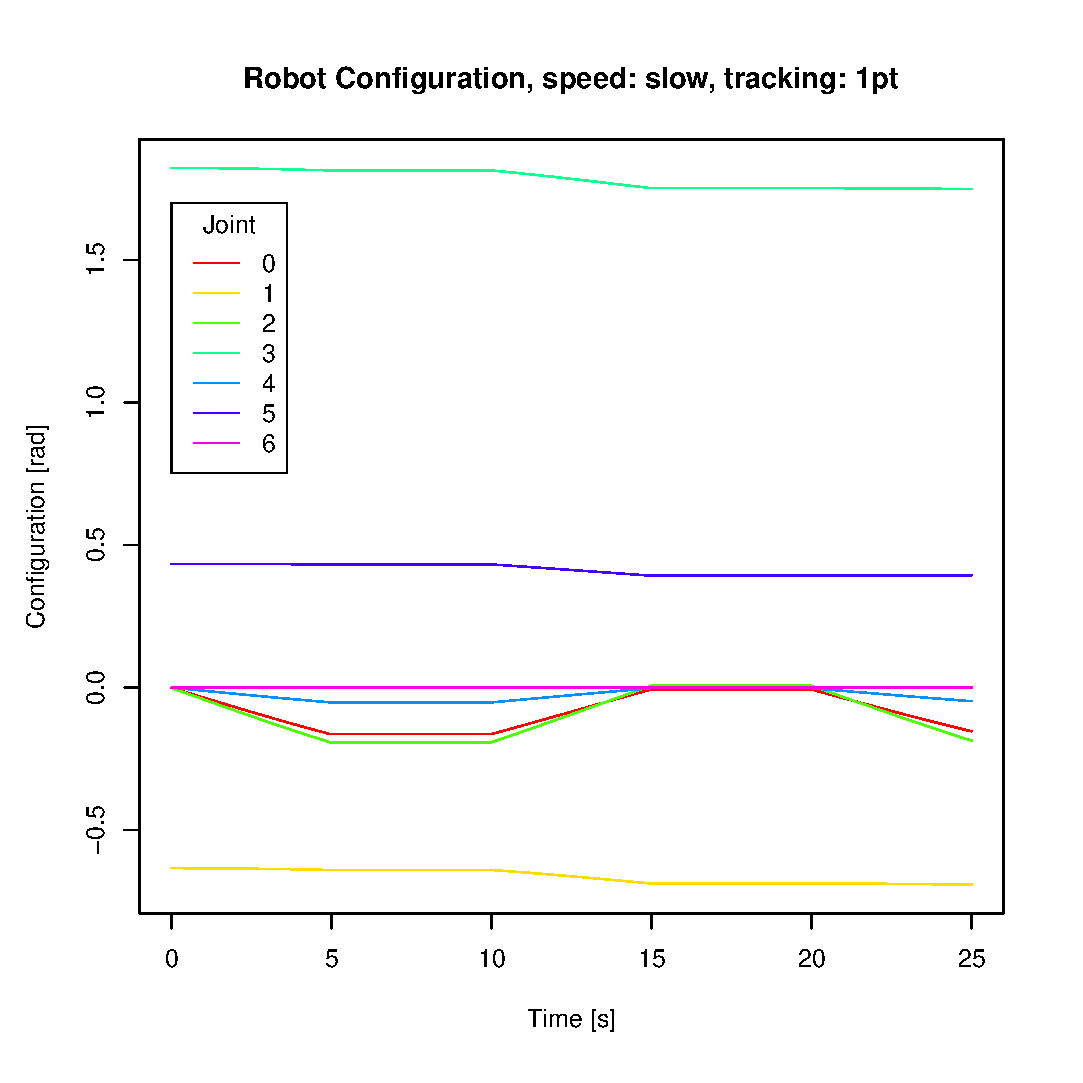
\includegraphics[width= \fullImageWidth]{graphics/robotics/robotConfiguration_slow_1pt}
\caption{Slow tracking speed of 3 points.}
\label{fig:robotic_conf_slow_1pt}
\end{figure}

\begin{figure}[H]
\centering
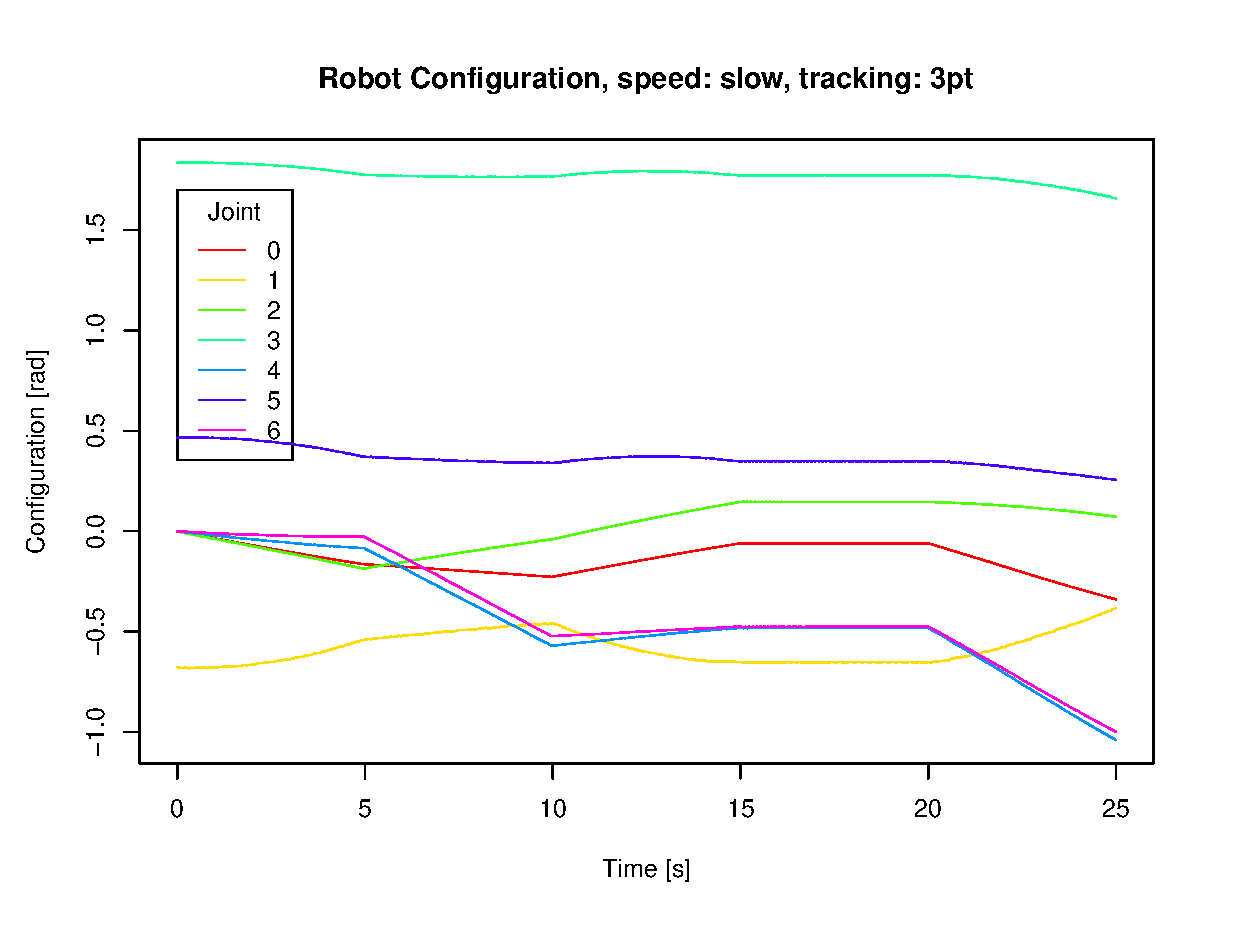
\includegraphics[width= \fullImageWidth]{graphics/robotics/robotConfiguration_slow_3pt}
\caption{Slow tracking speed of 3 points.}
\label{fig:robotic_conf_slow_3pt}
\end{figure}

\begin{figure}[H]
\centering
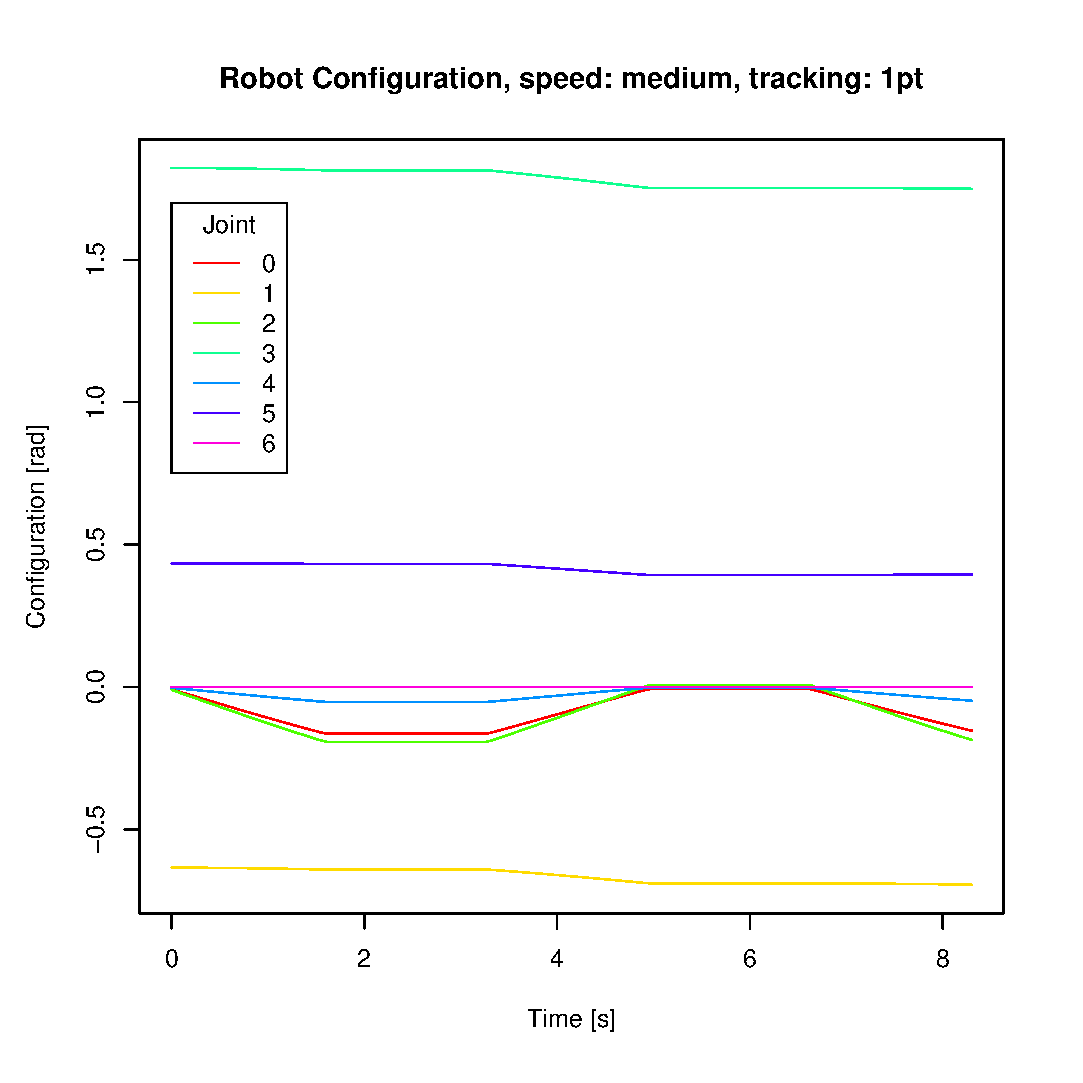
\includegraphics[width= \fullImageWidth]{graphics/robotics/robotConfiguration_medium_1pt}
\caption{Medium tracking speed of 3 points.}
\label{fig:robotic_conf_medium_1pt}
\end{figure}

\begin{figure}[H]
\centering
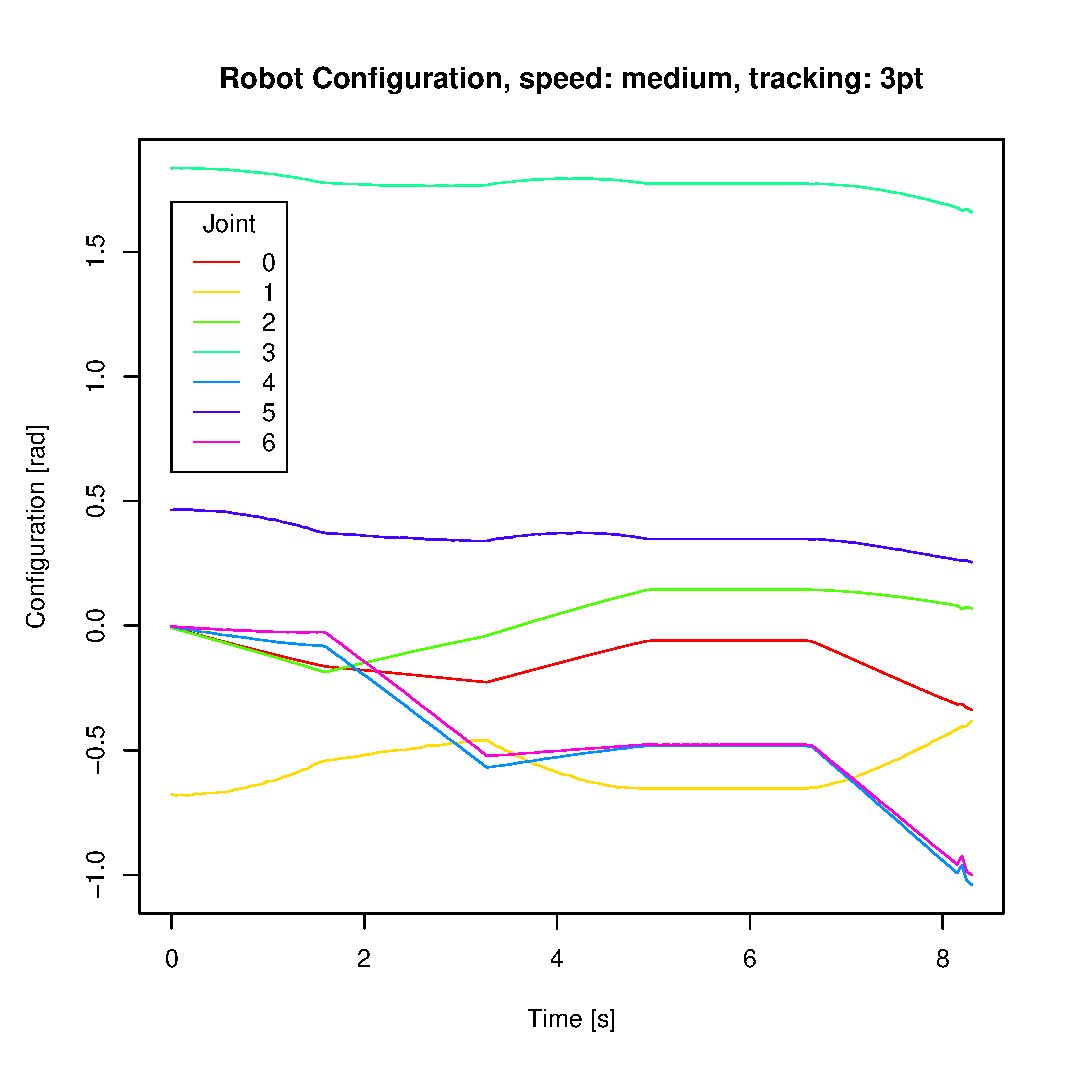
\includegraphics[width= \fullImageWidth]{graphics/robotics/robotConfiguration_medium_3pt}
\caption{Medium tracking speed of 3 points.}
\label{fig:robotic_conf_medium_3pt}
\end{figure}

\begin{figure}[H]
\centering
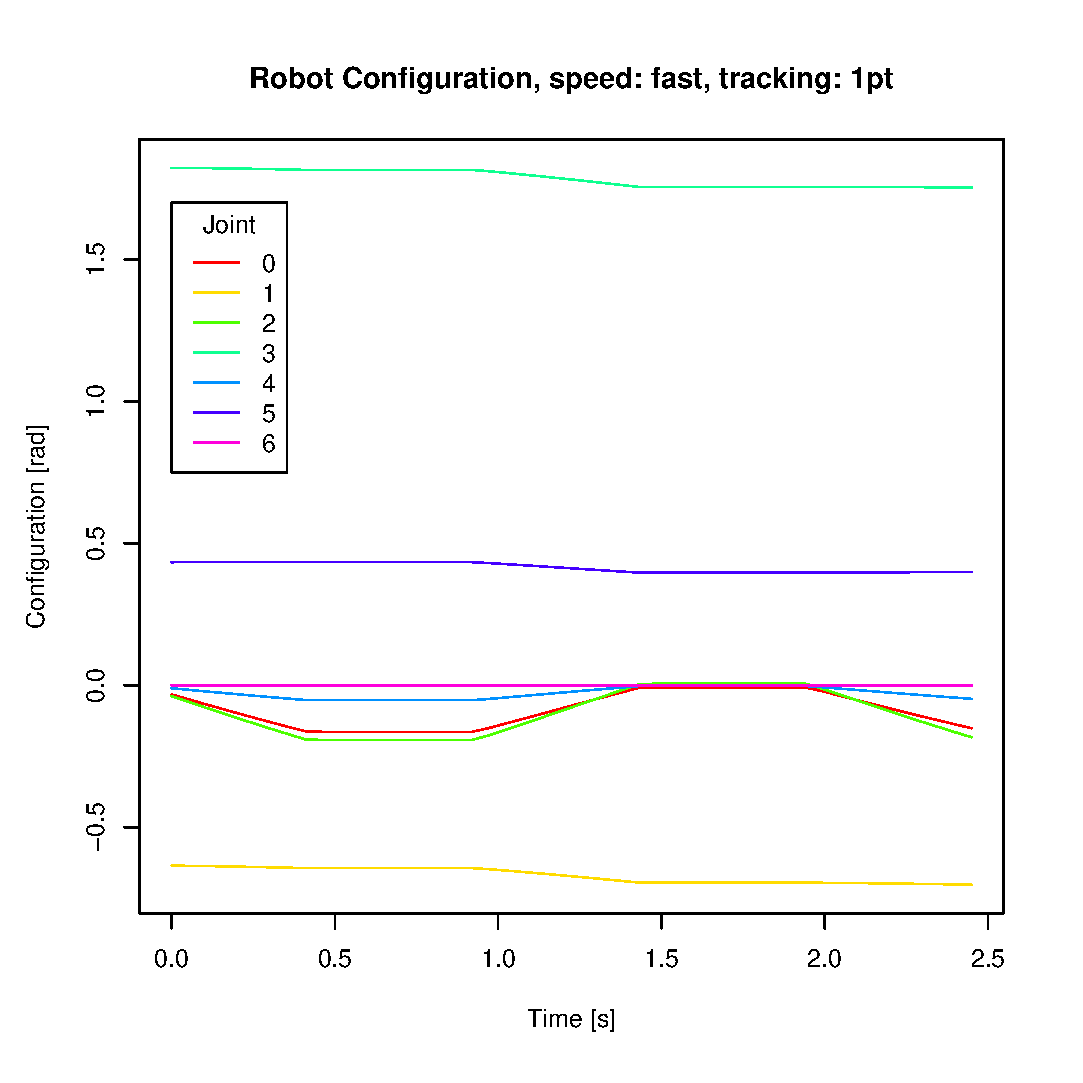
\includegraphics[width= \fullImageWidth]{graphics/robotics/robotConfiguration_fast_1pt}
\caption{Fast tracking speed of single point.}
\label{fig:robotic_conf_fast_1pt}
\end{figure}

\begin{figure}[H]
\centering
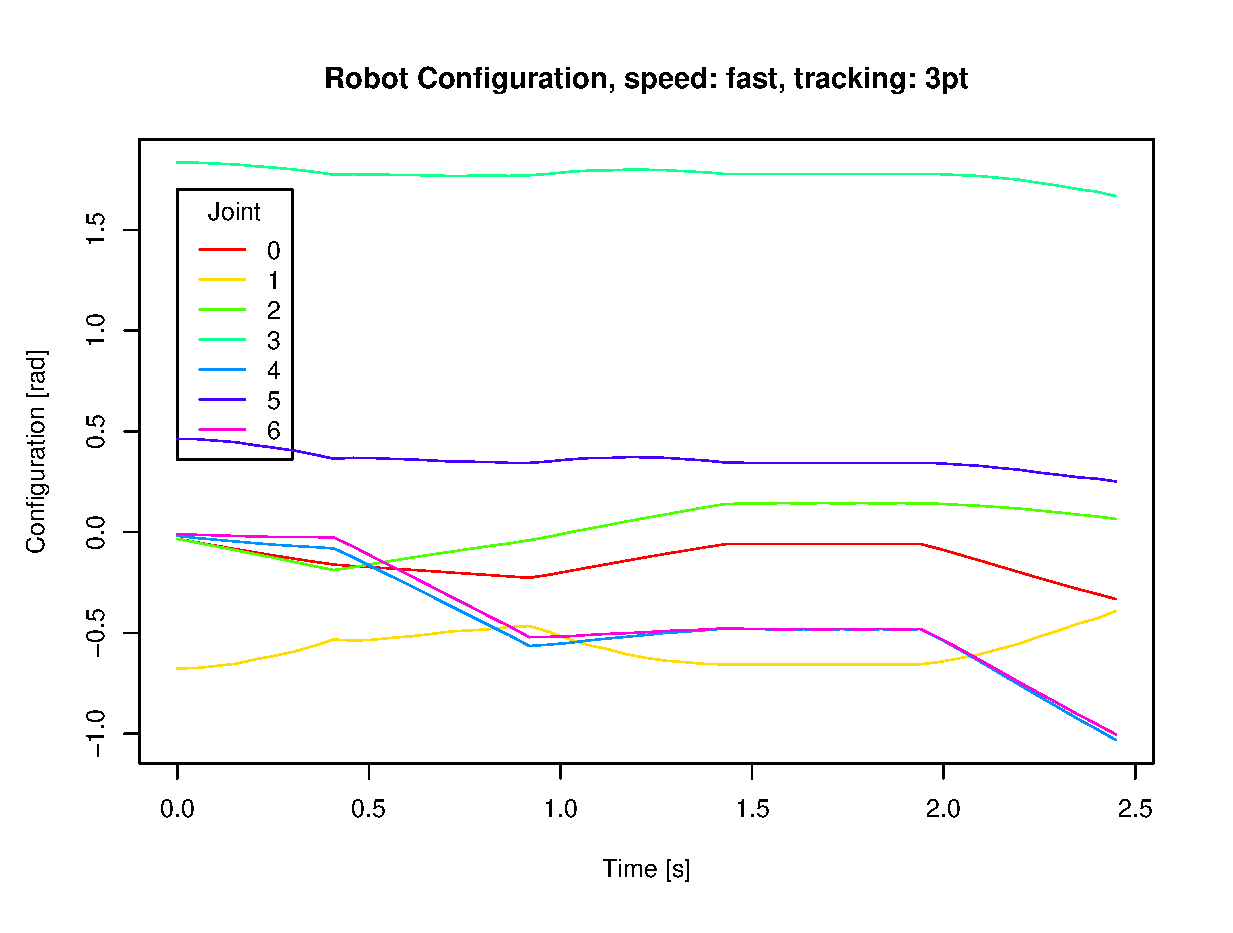
\includegraphics[width= \fullImageWidth]{graphics/robotics/robotConfiguration_fast_3pt}
\caption{Fast tracking speed of 3 points.}
\label{fig:robotic_conf_fast_3pt}
\end{figure}


